\chapter{Introduction}

This User Guide provides a guideline for the configuration and integration of the ETAS developed RTA-SUM SrvcMgr. RTA-SUM SrvcMgr module has been developed towards the Software Defined Veichle requirements, specifically, the SDV-8201 specifications and related specifications listed in Section \ref{sec:GBReferences}.

\ifnum \DocumentGroup=1
{
General guidelines on the common steps and workflow for RTA-SUM integration can be found in RTA-SUM Getting Started Guide.
}
\else
{
%Nothing
}\fi

\section{Definitions and Abbreviations}
\input{generated/tables/definitions.tex}

\section{Module Overview}
The Standard Utility Module Service Manager (SUM\_SrvcMgr) is a software component located in the Application Layer of the standardized architecture of AUTOSAR.

\textbf{SUM\_SrvcMgr} implements the following funtionalities:
\begin{enumerate}
\item Service Discovery Persistent Learning Session triggering.
\item Retrieval of learning table status and content.
\item Service Calibration Support: Capability of calibrating off services or service groups at initialization time.
\item Service status management at runtime based on specific project conditions.
\item Support SUM\_SPM to activate or deactivate services based on profile dependencies.  
\end{enumerate}

\begin{figure}[h!]
\centering
	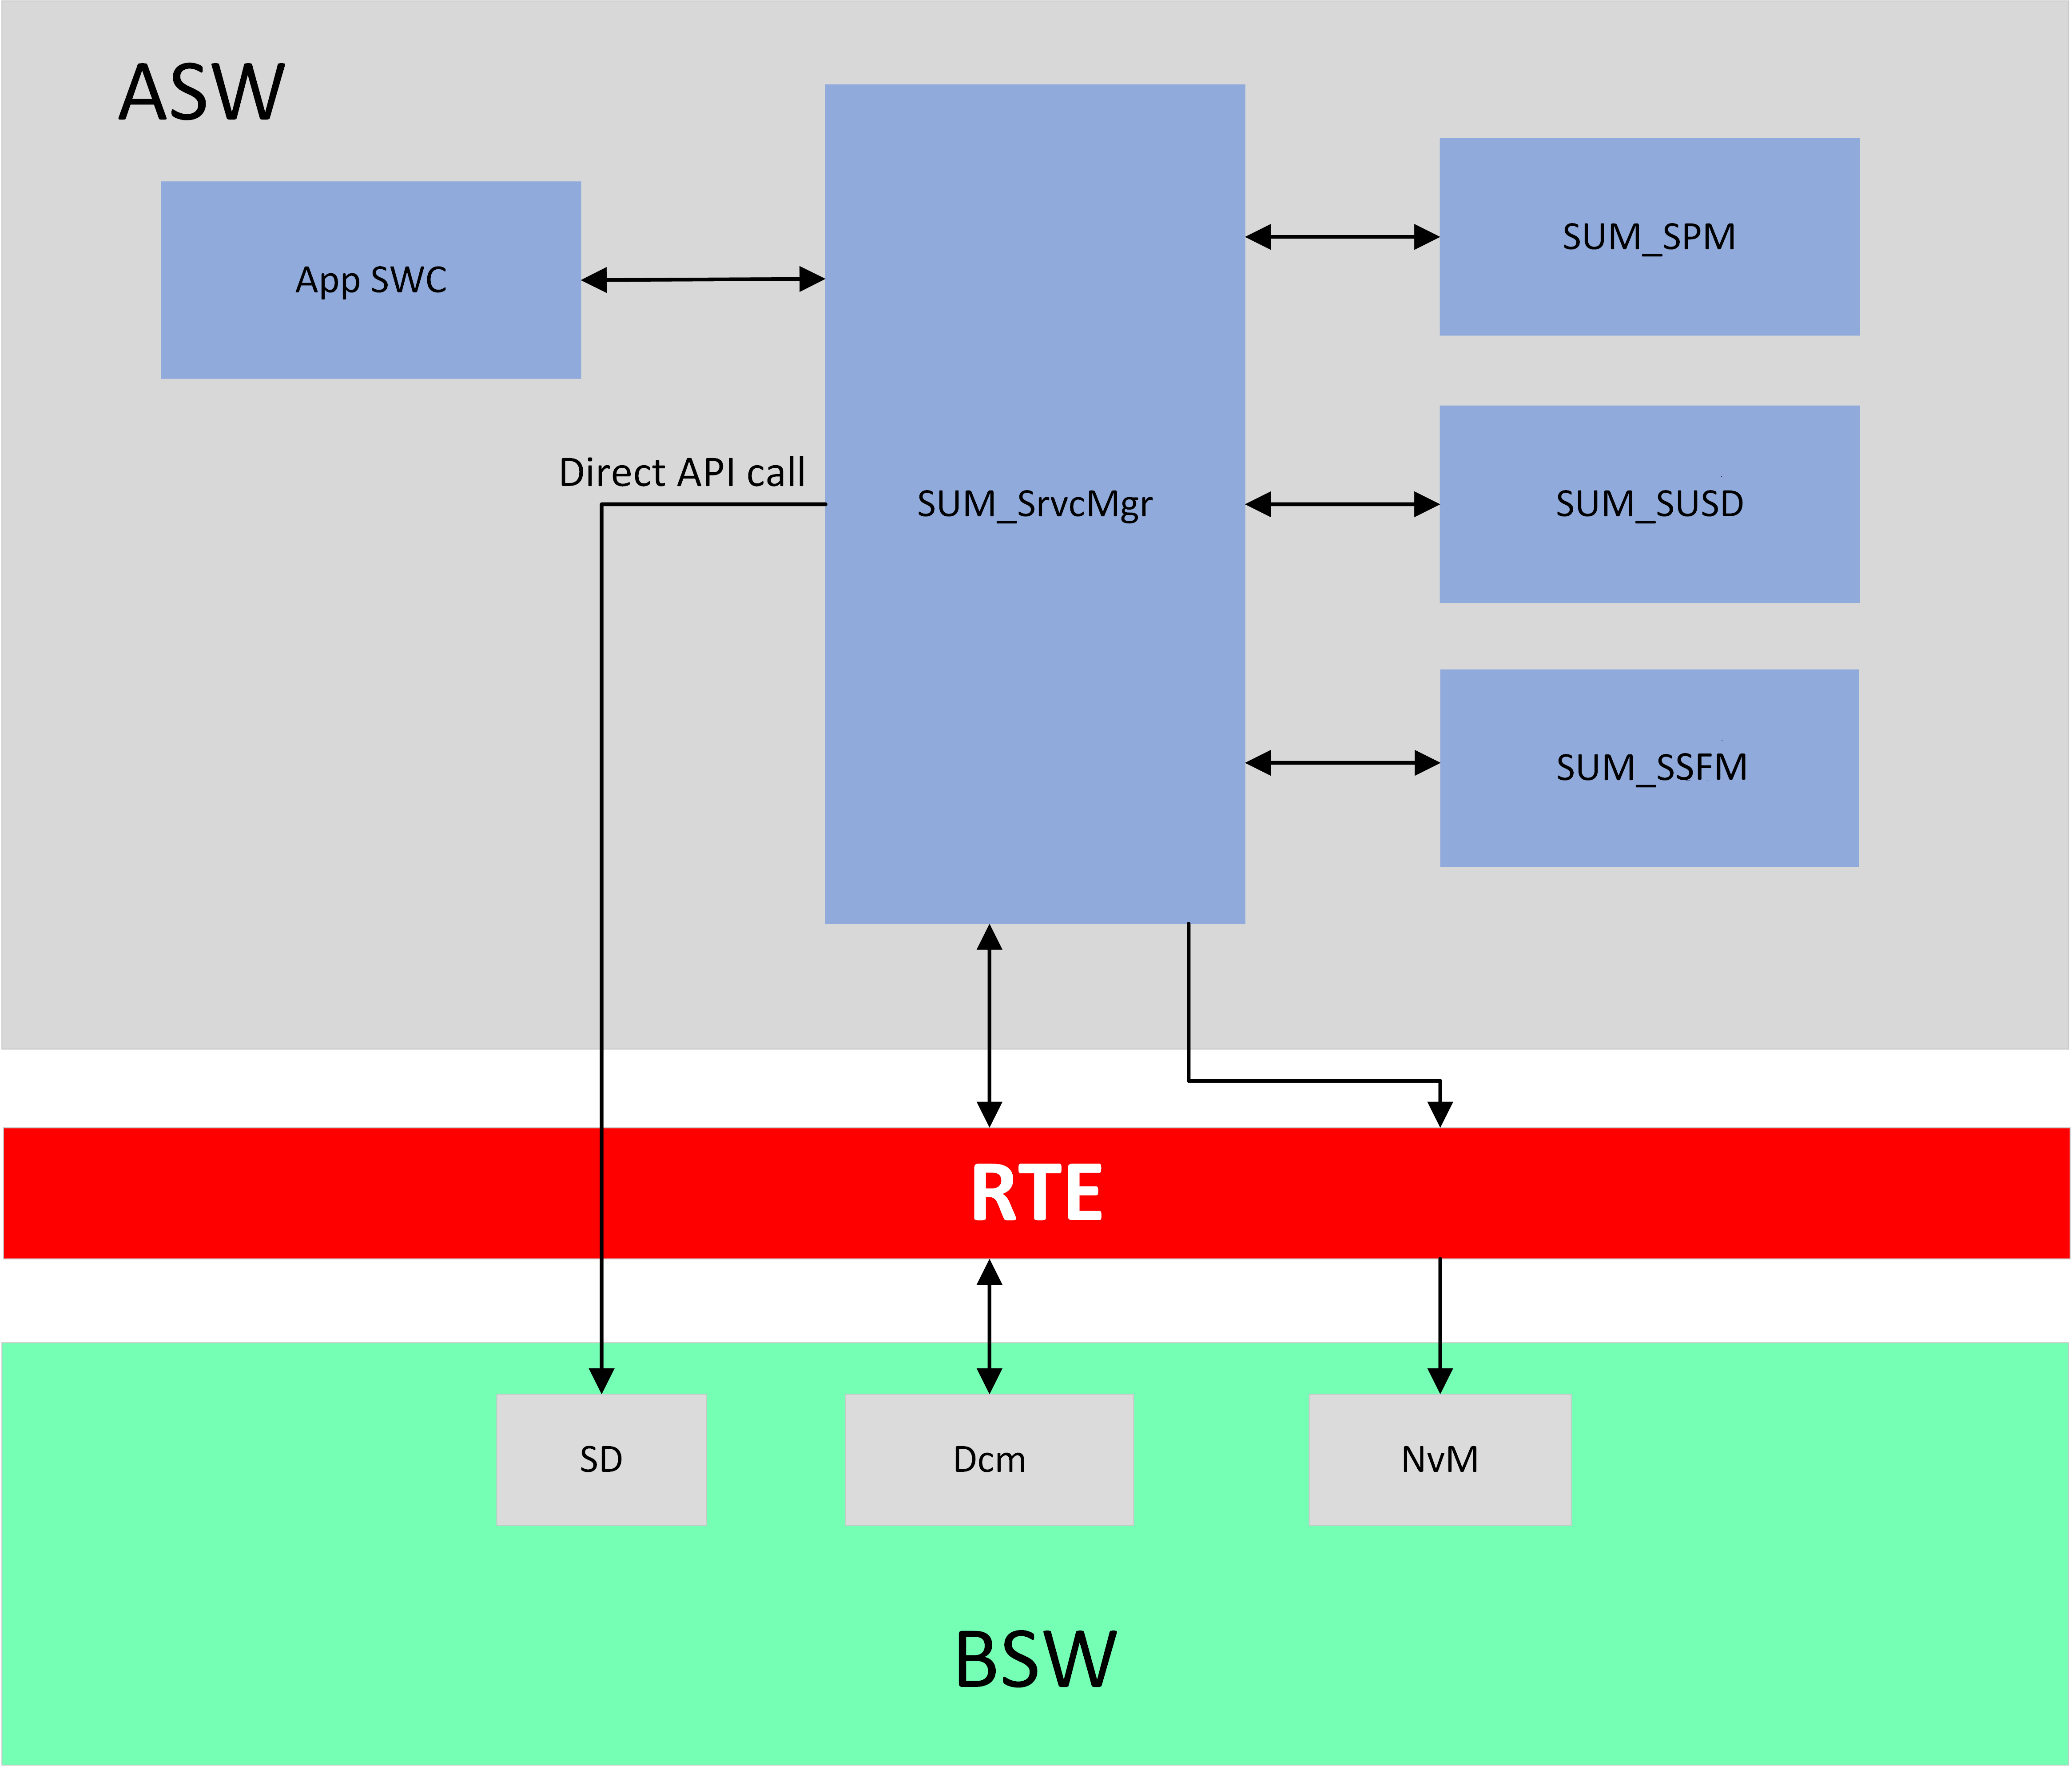
\includegraphics[scale=0.7]{images/SrvcMgr_System_Block_View.png}
	\caption{System layer overview.}
	\label{fig:Layers}
\end{figure}

\hfill \break


\section{References}
\label{sec:GBReferences}
\input{generated/tables/references.tex}
